\documentclass{article}
\usepackage[utf8]{inputenc}
\usepackage[]{hyperref}
\usepackage{float}
\usepackage[left=3cm, right=3cm, top=3cm]{geometry}
\usepackage{graphicx}
\begin{document}

\begin{center}
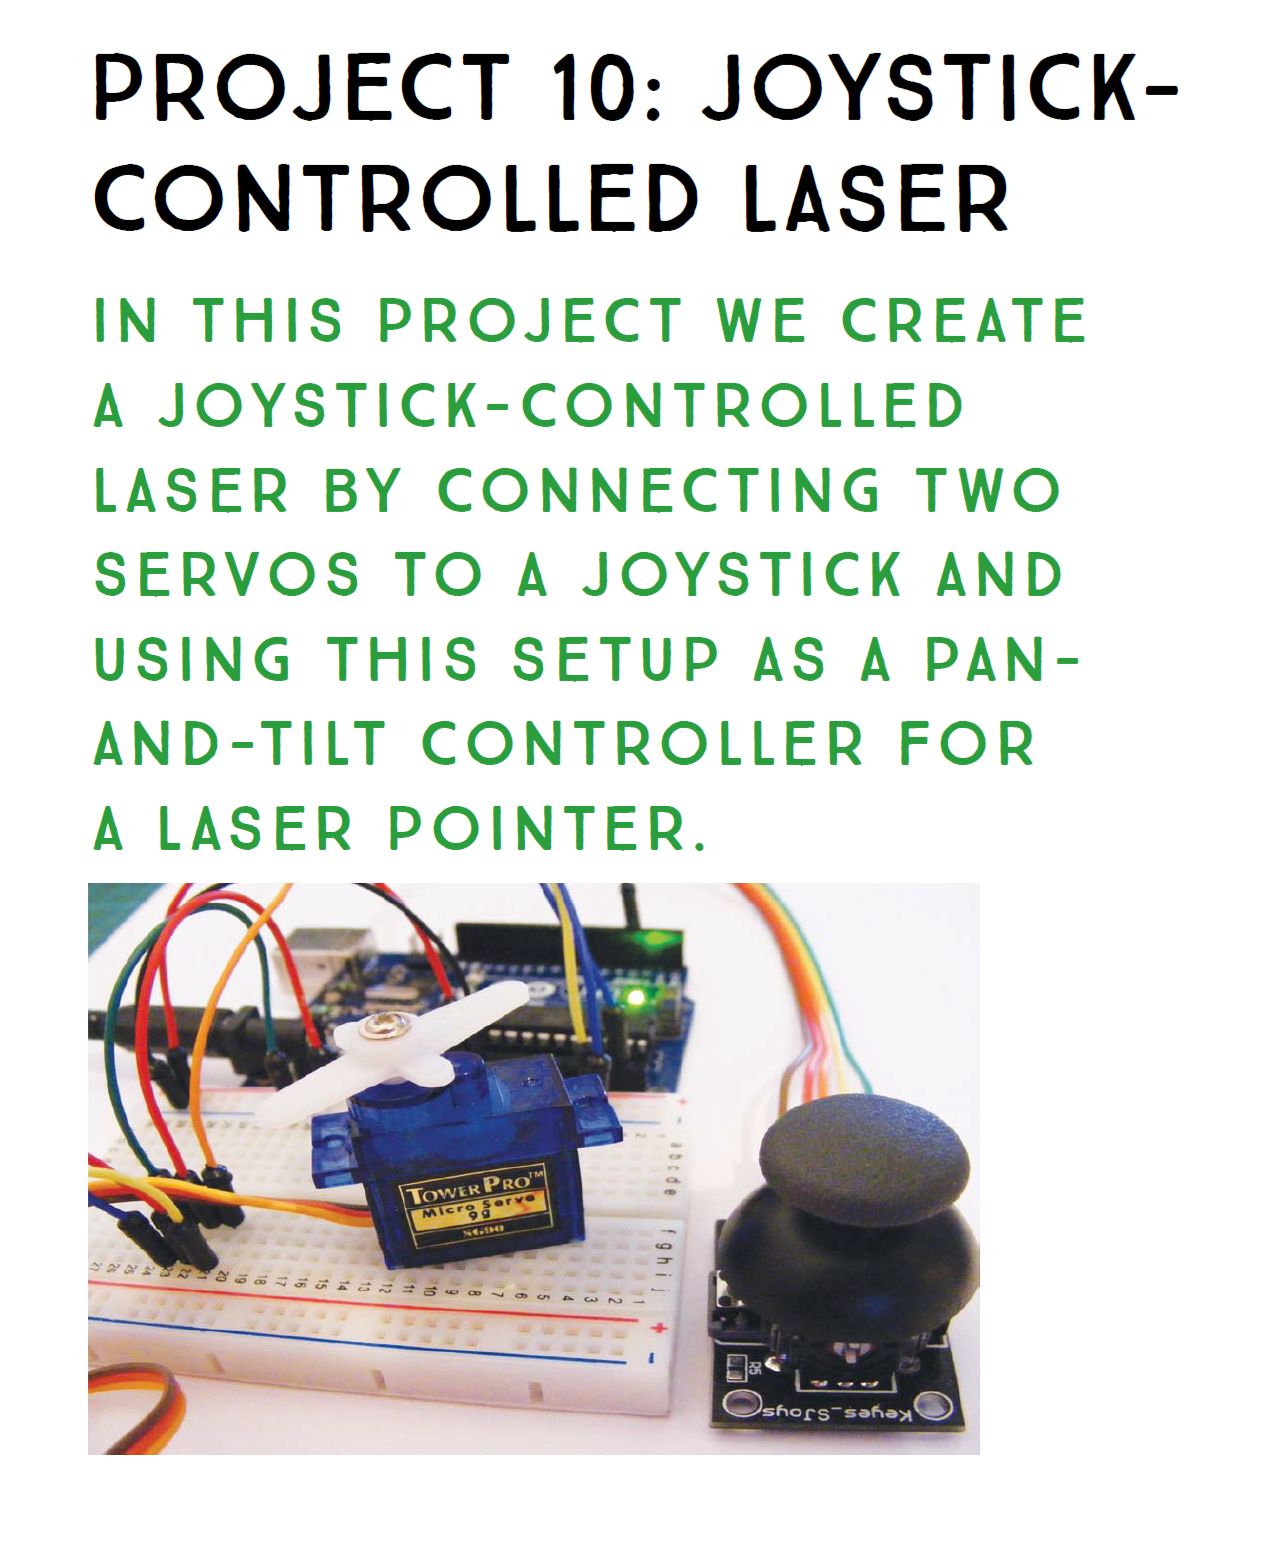
\includegraphics[width=\textwidth, height=20cm]{figures/title.png}
\end{center}

\section{Objectives}
By the end of this session, students should be able to:

\begin{itemize}
\item Describe the mechanical, electrical, and programming parts of joysticks and servos at a high
  level to someone unfamiliar with them.
\item Understand how pushbuttons work, what it means to ``debounce'' a pushbutton,
  and why debouncing is necessary in many cases.
\end{itemize}

\section{Parts Required}\label{sec:parts}
 (Approximate pictures of parts are in Fig.~\ref{fig:required-parts} below).

 \begin{figure}[H]
   \centering
   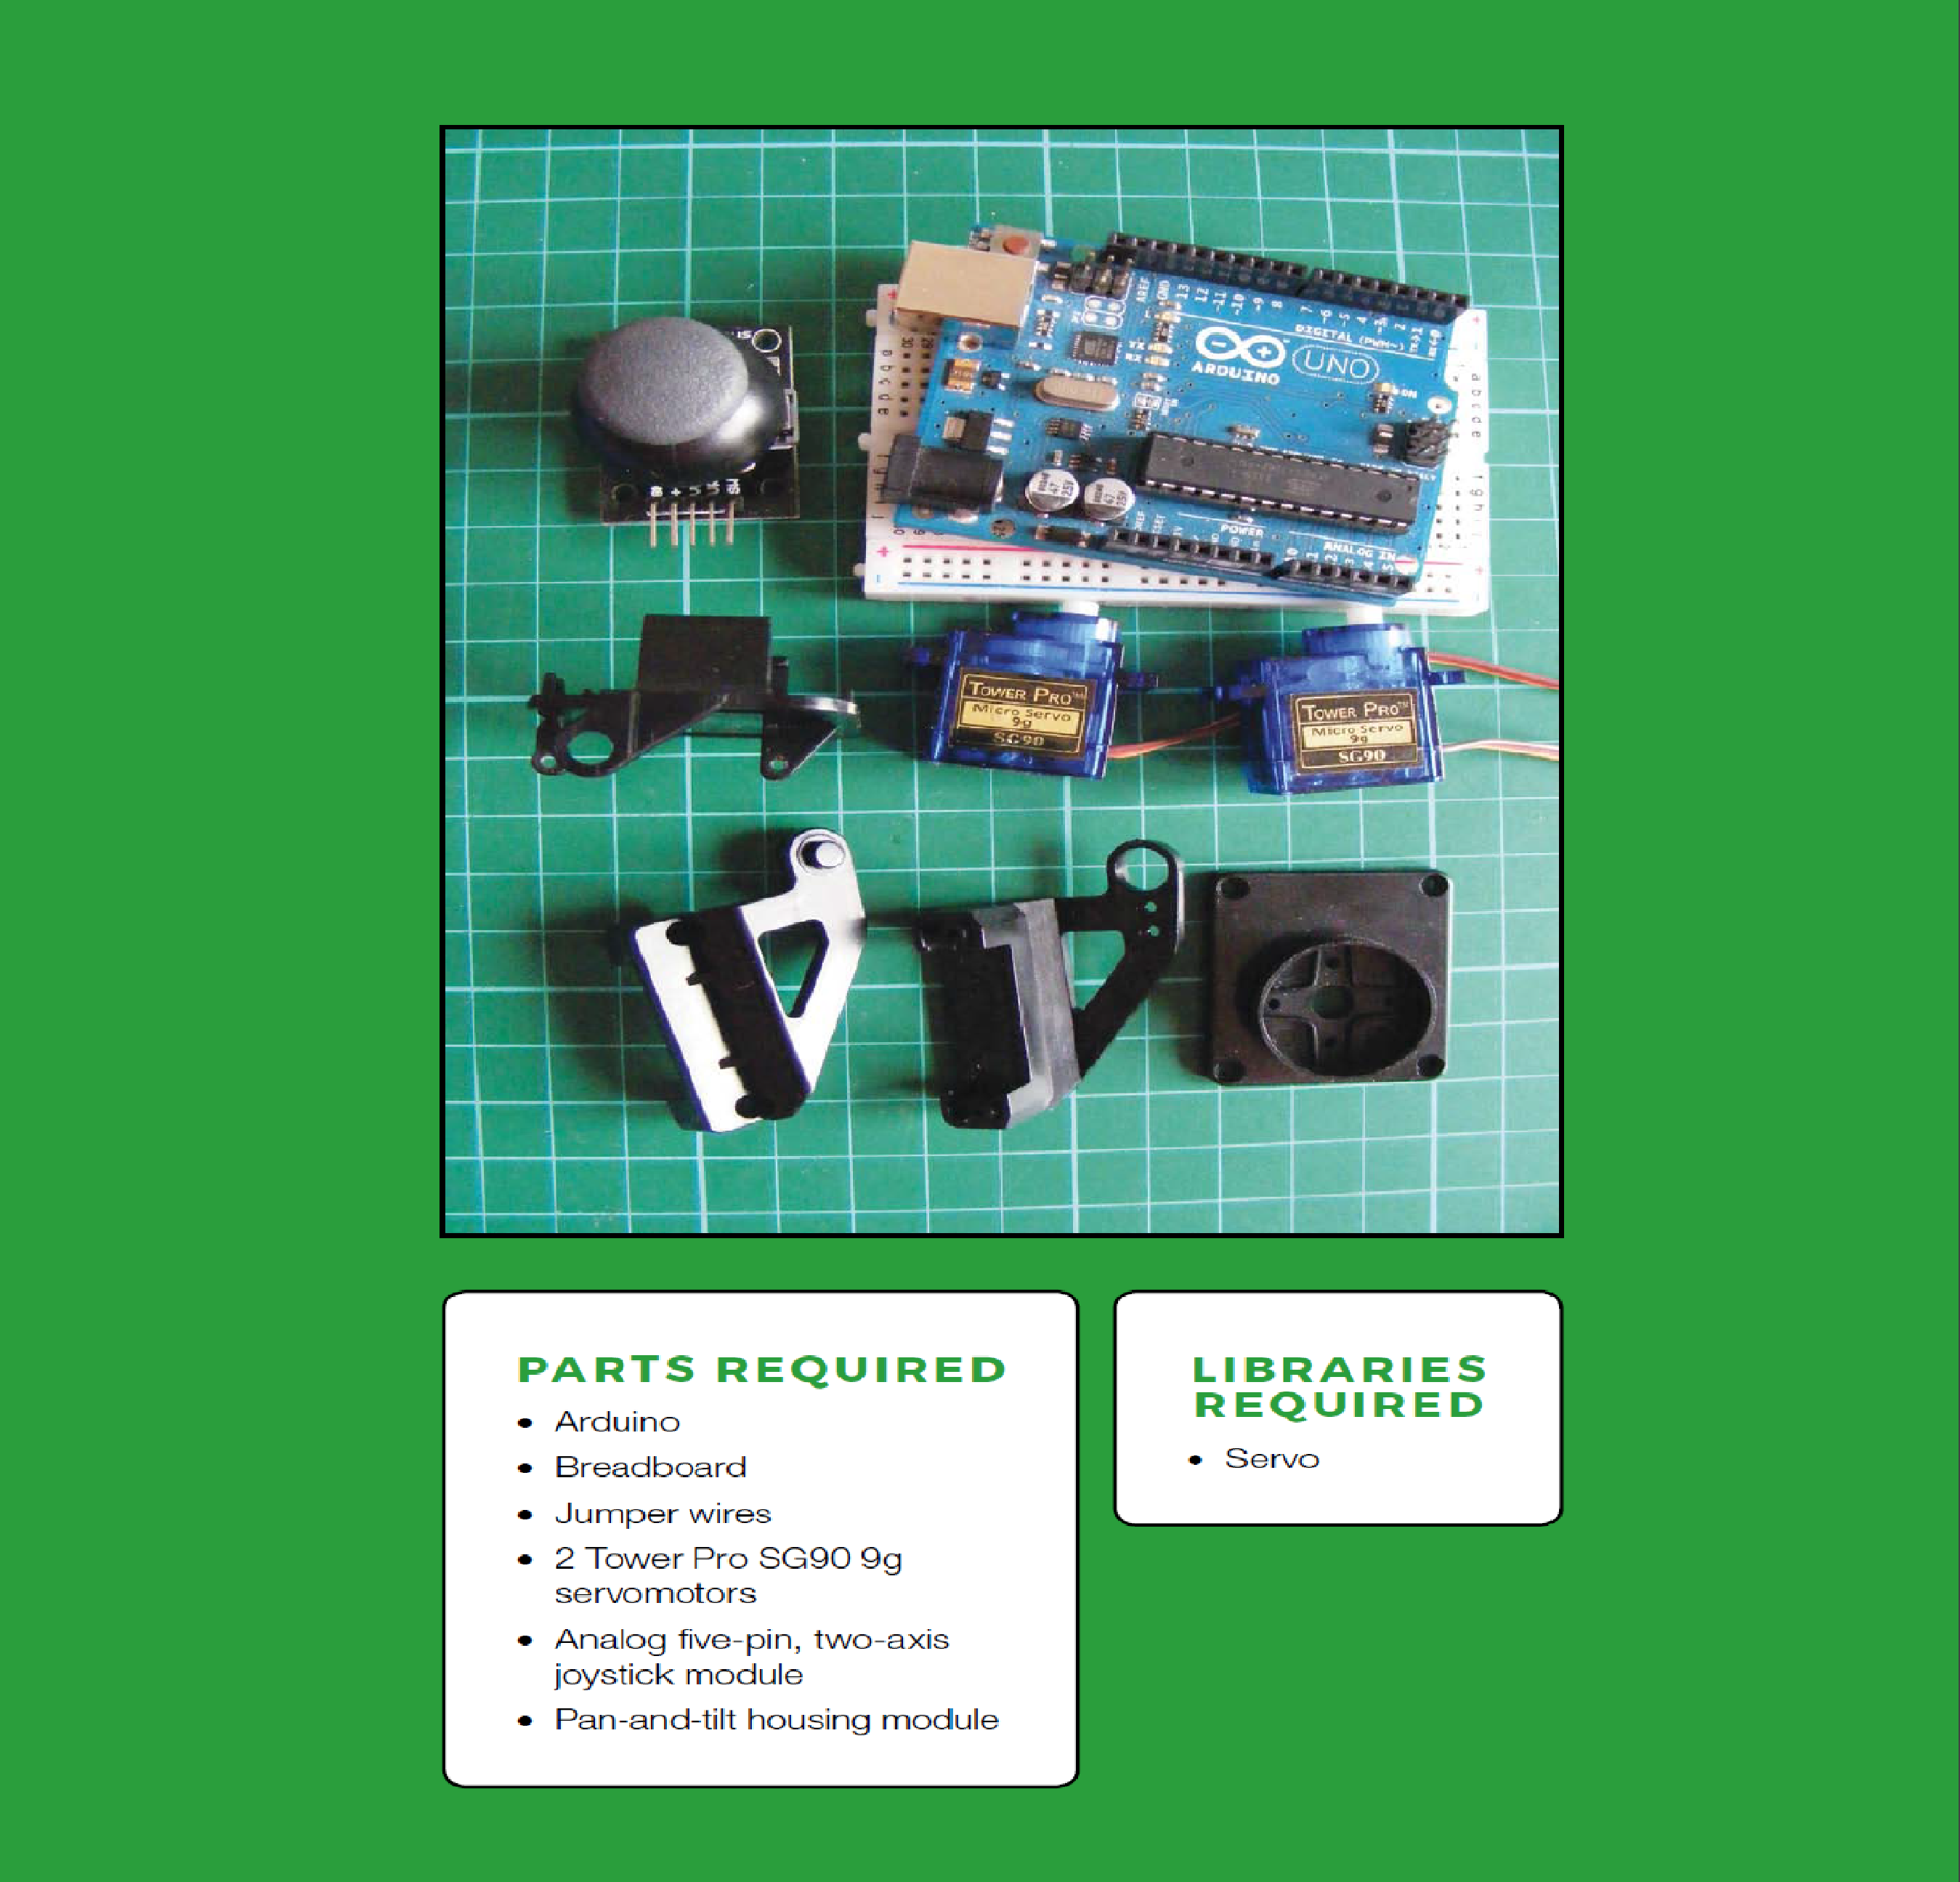
\includegraphics[width=.7\linewidth]{figures/required-parts.png}
   \caption{\label{fig:required-parts}}
 \end{figure}

 \section{Setup}
\begin{enumerate}
\item {Download, unzip, and install the Arduino Integrated Development Environment
    (IDE) from \href{https://www.arduino.cc/en/Main/Donate}{here} (does not need
    admin privileges). }
\item {Gather all of the parts listed in Section~\ref{sec:parts}}.
\item You will need to install the required \verb|Servo| library in the Arduino IDE
  by doing Tools->Manage Libraries, searching for the \verb|Servo| library and then
  clicking the install button.
\end{enumerate}

\section{How it Works}
Servos are small motors that can precisely angle their arms to positions between 0
and 180 degrees (like your forearm+elbow can!). In this project you will be working
with two servos that have been placed into a tilt-and-pan mount: one for motion to
the left or right, and one for motion up and down. Because the tilt-and-pan mount
contains two servos, it can move through 180 degrees in two directions, and we say it
has \emph{two} degrees of freedom (out of six total possible).

\begin{figure}[H]
  \centering
  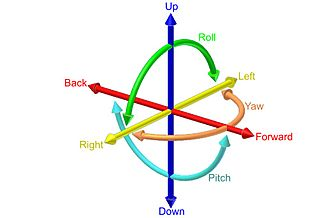
\includegraphics[width=.7\linewidth]{figures/roll-pitch-yaw.jpg}
  \caption{\label{fig:roll-pitch-yaw}}
\end{figure}

More precisely, out of the six possible degrees of freedom in
Fig.~\ref{fig:roll-pitch-yaw}, we will be controlling the ``pitch'' and ``yaw'' axes
with our joystick, and our laser (which will be attached to the tilt-and-pan mount)
will be able to move around quite a bit.

The other piece of hardware we will be using is 2D joystick (2D = two degrees of
freedom = X and Y axis tracking). Our joystick is basically just two potentiometers
(one per axis) that all us to measure the movement of the stick all each axis
independently. Potentiometers are variable resistors that know their value, which for
our joystick is between 0 and 1,023. As you move the joystick around its center in X
and Y, the potentiometers measure the resistance between the current position of the
``stick'' for each axis between a voltage source and ground, and report that to the
Arduino, which then decides how far the servos move, as shown in
Fig.~\ref{fig:joystick-output}. Our joystick also has a multi-purpose button we will
be using for turning the laser on and off.

\begin{figure}[H]
  \centering
  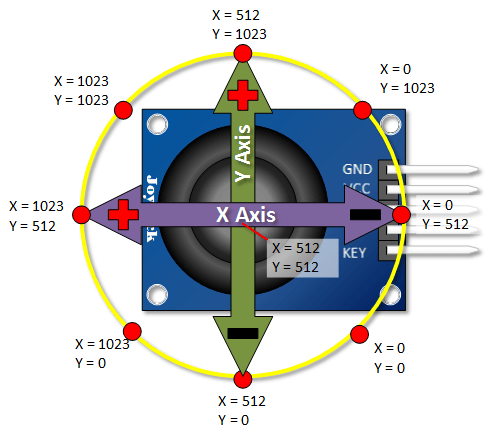
\includegraphics[width=.7\linewidth]{figures/joystick-output.png}
  \caption{\label{fig:joystick-output}}
\end{figure}

When the joystick is moved to the left or right, the corresponding servo will move in
that direction; when the joystick is moved up or down, the other servo will move up
or down. When you are using the joystick, it should feel familiar---most video game
controllers have joysticks very similar to this one, and they all work basically the
same way!

\section{Building the Circuits}
IMPORTANT! When building circuits on breadboards which holes are linked together
matters a lot! Not all rows/columns of circuits are connected. See the diagrams below
for an explanation of which holes are connected. The \emph{vertical} columns along
the edges of the breadboard are connected, and the \emph{horizontal} rows in the
middle part of the breadboard are connected. But, both the horizontal row and the
vertical column connections do not cross the central line.

    \begin{figure}[H]
      \centering
      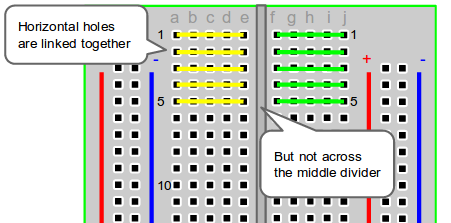
\includegraphics[width=\textwidth]{figures/breadboard-connectivity1.png}
      \caption{\label{fig:breadboard-connectivity1}}
    \end{figure}

    \begin{figure}[H]
      \centering
      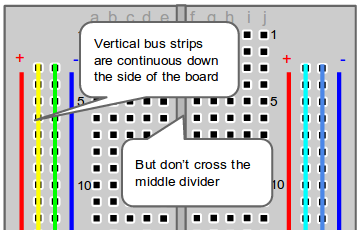
\includegraphics[width=\textwidth]{figures/breadboard-connectivity2.png}
      \caption{\label{fig:breadboard-connectivity2}}
    \end{figure}

\begin{enumerate}
\item {Connect the servos and the joystick to the Arduino, as shown in
    Fig.~\ref{fig:diagram}. Note that the \emph{brown} wire on the servo is ground,
    the \emph{red} one is power, and the \emph{yellow-orange} one is the input signal
    to the Arduino.

    \begin{figure}[H]
      \centering
      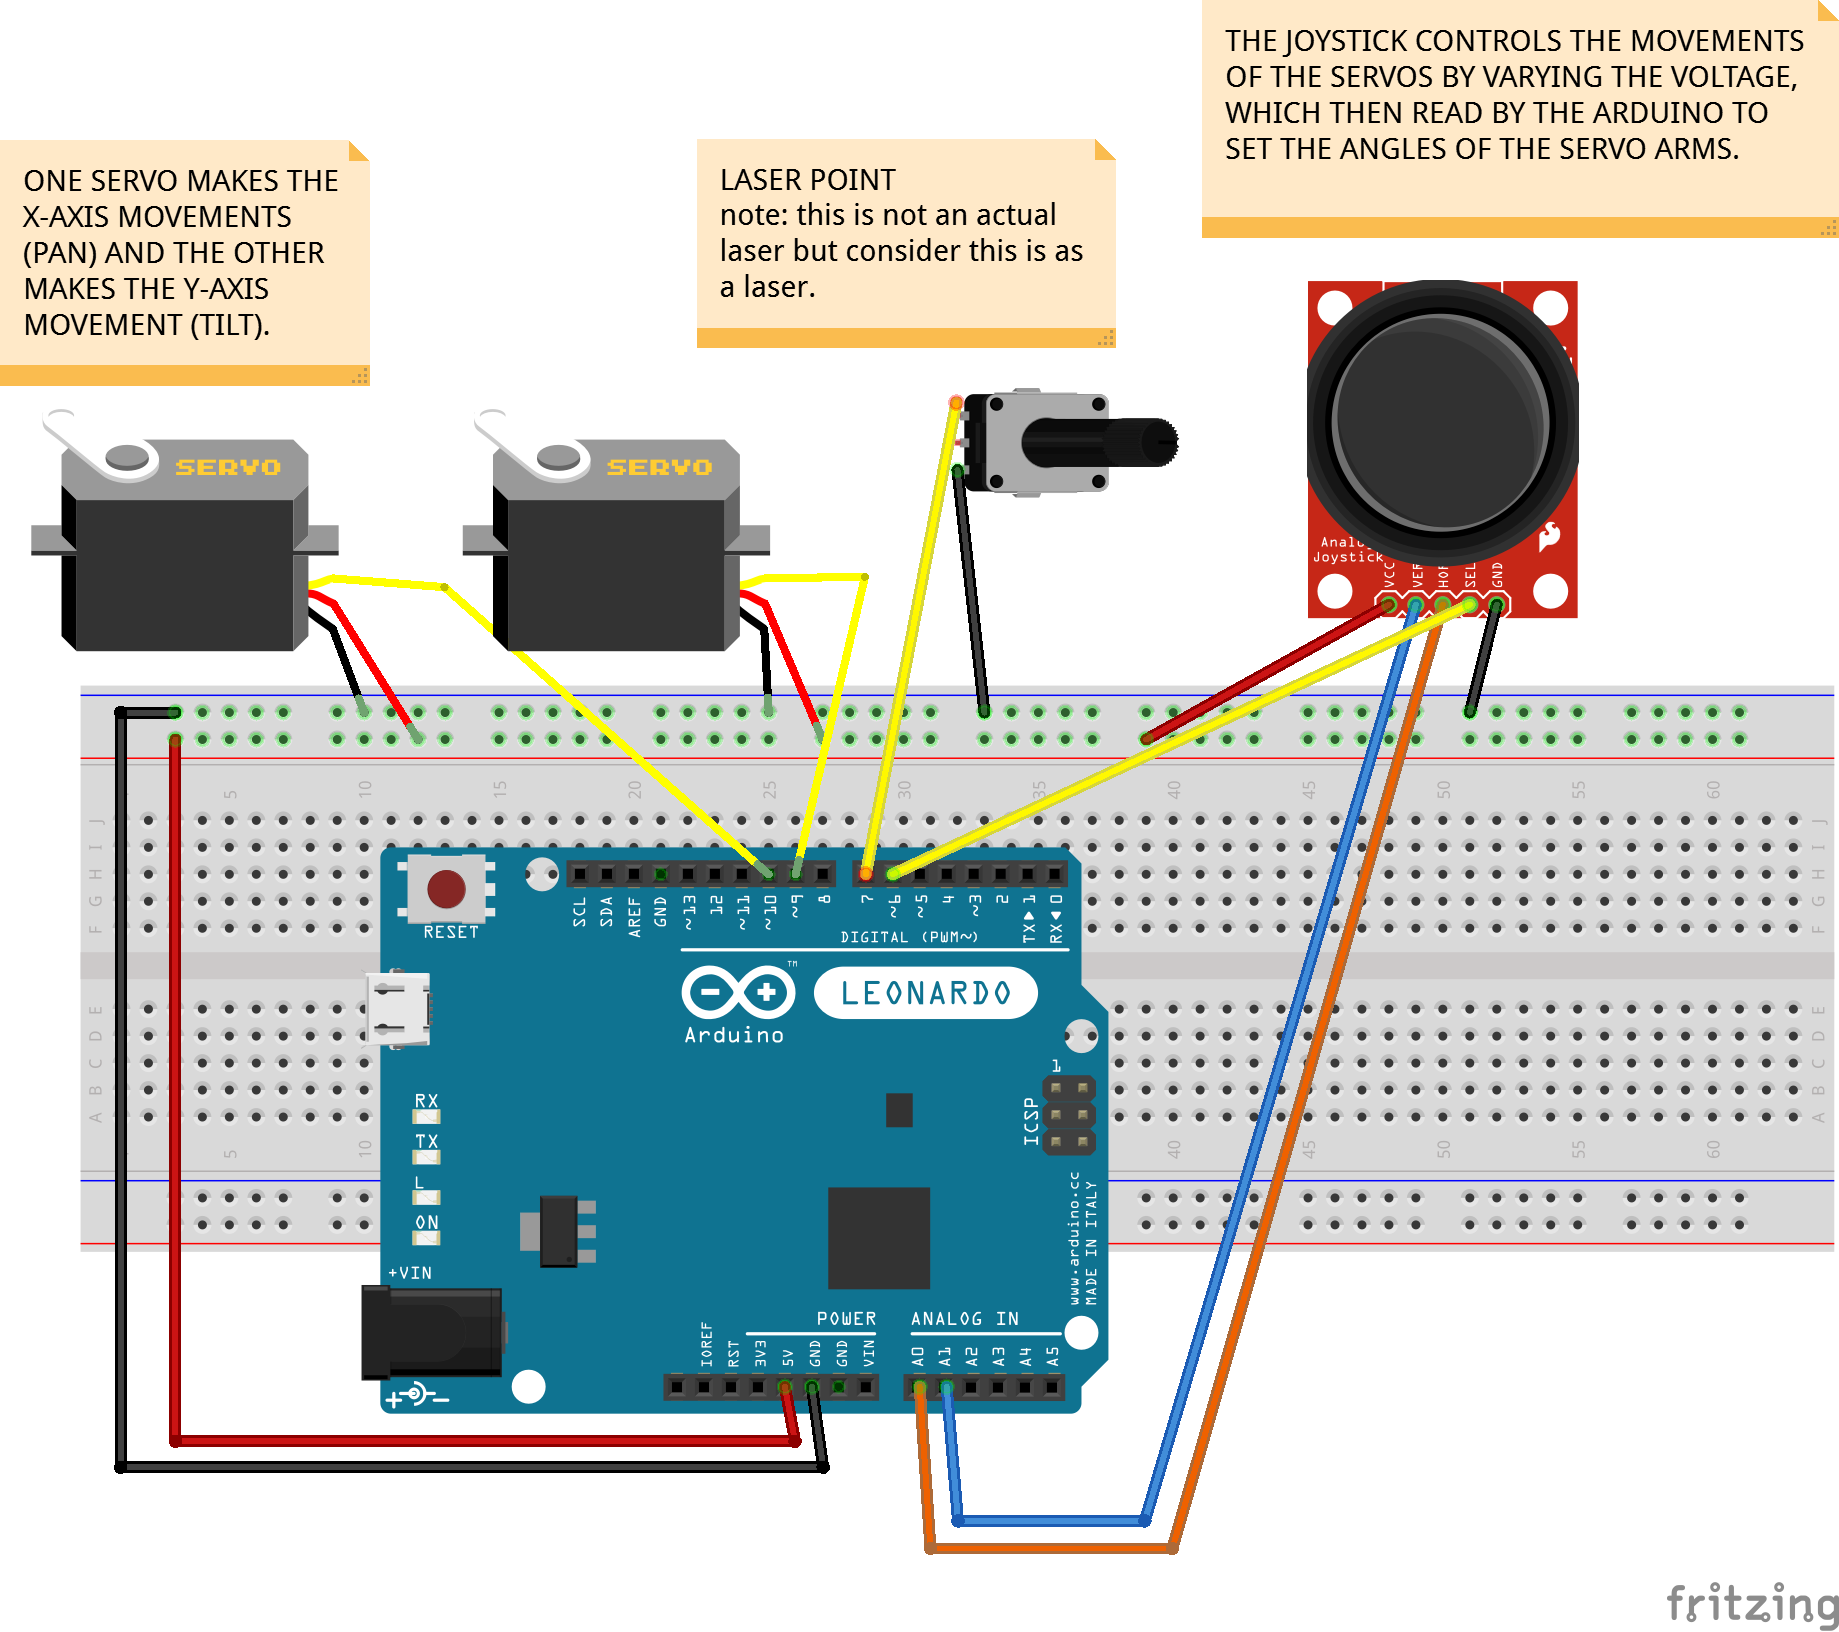
\includegraphics[width=\textwidth]{figures/diagram.png}
      \caption{\label{fig:diagram}}
    \end{figure}
  }
\item {Attach the laser diode to the top of the module using masking tape. You will
    also want to tape the tilt-and-pan module to the table so the laser will be
    stable when you move it around. Now you can control the laser using the joystick!
    To turn the laser on/off, you can push the joystick like it is a button (you will
    here a slight click). If it doesn't work very well, don't worry! Read on and you
    learn why.}
\end{enumerate}
  
\section{Programming the Arduino}
The base code for programming the Arduino is provided. Using the Arduino IDE, open
the .ino file.  The IDE allows you to do 4 things: edit the code, verify the code
(i.e.~does not contain syntax errors), upload the code to the Arduino, and view the
diagnostic output of things as they run on the Arduino.  Uploading to the Arduino is
easy! Just click the Upload arrow in the IDE.

\section{Understanding the Code}
There are two main sections of code whenever you use an Arduino: \verb|setup()| and
\verb|loop()|. The \verb|setup()| code runs once when you first load the sketch (or
turn the Arduino on), and the \verb|loop()| code runs over and over without stopping
until you load a different sketch onto the Arduino or turn it off.

In the \verb|setup()| section, we tell the Arduino that the laser on/off will be
controlled by the Arduino, and is an \emph{output}, the button on the joystick is an
\emph{input} into the Arduino sketch. Finally, we tell the Arduino where the joystick
inputs will be coming from: the joystick x-axis is attached to Arduino pin A0 and the
y-axis to Arduino A1, and these are our analog \emph{inputs} (the variable resistors we
learned about earlier). The x- and y-axes are then set as variables for movement.

The ``pitch'' servo is attached to Arduino pin 9 and ``yaw'' is attached to Arduino
pin 10, and these are our \emph{output}. The Arduino then reads the \emph{input} from
the joystick and changes this voltage to \emph{output}, moving the servos according
to which direction is chosen.

\section{ Extending the Code}
Once you have the joystick-controlled laser working, try to press the button on the
joystick to turn on or turn off the laser. What happens when you try that? Kind of
jerky/inconsistent right?  We need to ``debounce'' the button we press, so that the
Arduino more reliably reads the correct state of the button from the
joystick. Debouncing is very common in embedded computing systems and works as
follows:

\begin{enumerate}
\item {Check the state of a button at a given time, and save this value as \emph{A}.}
\item {Check the state of a button a little bit later (``later'' in computer terms, in
    terms of real time it is < 100 ms!) and save this value as \emph{B}.}
\item {Treating the button as having been pressed (or released) if and only if
    \emph{A} and \emph{B} are the same (both ``pushed'' or both ``not pushed'').}
\end{enumerate}

Almost all electronic buttons you press do this in hardware or software, so that your
intent is clearly communicated to the program that is running.

There is already a function in the code that can perform debouncing, all you need to
do is to modify the code slightly to use it! How can you do so?

Once you have debouncing working, how about making the motion of the servos smoother?
It feels a little jerky/moves too far in either direction. How can you make the range
smaller? HINT: look at the usage of the \verb|map()| function.

\section{Going Further}
Now that you have mastered debouncing and making the motion of the servos a little
bit smoother, lets try adding a new component to our Arduino circuit, and try writing
some new code to use it. A common electronic component is the piezoelectric buzzer (a
sound making device capable of vibrating itself at different speeds to make different
musical notes). Try incorporating it into the Arduino circuit so that whenever the
laser is ON, the buzzer is ON too (sort of a safety warning mechanism to remind you
not to shine the laser into your eye!). To get an idea of how to incorporate it, look
at this
\href{https://create.arduino.cc/projecthub/SURYATEJA/use-a-buzzer-module-piezo-speaker-using-arduino-uno-89df45}{example}. The
basic steps are

\begin{enumerate}
\item Modify the physical circuit to incorporate the buzzer (you can attach it to any
  available digital pin on the Arduino).
\item Set the pin you connected it to as an \emph{output} in the \verb|setup()| code.
\item Add the \verb|tone()/noTone()| code in the \verb|loop()| as needed to turn the
  buzzer on and off in tandem with the laser.
\end{enumerate}
\end{document}
